\documentclass{article} % For LaTeX2e
\usepackage{nips14submit_e,times}
\usepackage{hyperref}
\usepackage{url}
\usepackage{amsmath,amsfonts,amsthm}
\usepackage{bbm}
\usepackage{algorithm,algorithmic}
\usepackage{graphicx}
\usepackage{bm}
\usepackage{bbm}
\usepackage[titletoc]{appendix}
\usepackage{wrapfig}
\usepackage{afterpage}
\usepackage{amssymb}
\usepackage{booktabs}
\usepackage{ulem}
\usepackage{multirow}
\usepackage{comment}

\def\B#1{\bm{#1}}
%\def\B#1{\mathbf{#1}}
\def\trans{\mathsf{T}}
\DeclareMathOperator*{\argmin}{arg\,min}

%\renewcommand{\labelitemi}{--}

\newtheorem{theorem}{Theorem} \newtheorem{lemma}[theorem]{Lemma}
\newtheorem{proposition}[theorem]{Proposition}
\newtheorem{corollary}[theorem]{Corollary}
\newtheorem{definition}[theorem]{Definition}
\newtheorem{remark}{Remark}

%%%%%%%%%%%%%%%%%%%%%%%%%%%%%%%%%%%%%%%%%%%%%%%%%%%%%%%%%%%%%%%%%%%%%%%%%%%%%%%

\title{Region-network hierarchical sparsity priors for\\
high-dimensional inference in brain imaging}

\newcommand{\fix}{\marginpar{FIX}}
\newcommand{\new}{\marginpar{NEW}}
\DeclareMathOperator{\proj}{proj}
\DeclareMathOperator{\softmax}{softmax}
\DeclareMathOperator{\prox}{prox}
\DeclareMathOperator{\Prox}{Prox}
\DeclareMathOperator{\im}{im}

% macros from michael's .tex
\DeclareMathOperator{\dist}{dist} % The distance.
\DeclareMathOperator{\argmin}{argmin}
\DeclareMathOperator{\argmax}{argmax}
\DeclareMathOperator{\Id}{Id}
\DeclareMathOperator{\abs}{abs}
\newcommand{\R}{\mathbb{R}}
\newcommand{\N}{\mathbb{N}}
\newtheorem{thm}{Theorem}[section]
\newtheorem{prop}[thm]{Proposition}
\newtheorem{lem}[thm]{Lemma}
\newtheorem{cor}[thm]{Corollary}


\newcommand{\suggestadd}[1]{{\color{blue} #1}}
\newcommand{\suggestremove}[1]{{\color{red} \sout{#1}}}

% \nipsfinalcopy % Uncomment for camera-ready version
\nipsfinaltrue
%%%%%%%%%%%%%%%%%%%%%%%%%%%%%%%%%%%%%%%%%%%%%%%%%%%%%%%%%%%%%%%%%%%%%%%%%%%%%%%

\begin{document}

\author{Danilo Bzdok, Michael Eickenberg,
  Ga\"el Varoquaux, Bertrand Thirion\\
  Department of Psychiatry, Psychotherapy and Psychosomatics, RWTH Aachen, Germany\\
  INRIA, Parietal team, Saclay, France\\
  CEA, Neurospin, Gif-sur-Yvette, France\\
  firstname.lastname@inria.fr}

\maketitle

\begin{abstract}
% Imaging neuroscience links human behavior to aspects of brain
% biology in ever-increasing datasets.


\textbf{\\keywords}:
Sparsity-inducing norms, hierarchical structured sparsity,
numerical optimization,
systems neuroscience, brain imaging,
functional specialization, functional integration

\end{abstract}



\section{Introduction}
% sparsity
Many quantitative scientific domains underwent a
recent passage from the classical regime (i.e., "long data")  to
the high-dimensional regime (i.e., "wide data")
\cite{jordan2015massive}.
Also in the brain imaging domain,
many contemporary methods for acquiring brain signals yield
more variables per observation than
total observations per data sample.
This high-dimensional scenario challenges many statistical estimators from
classical statistics.
For instance,
the general linear model without additional assumptions
yields an infinity of possible coefficients
and, thus, no solution.
%
Many such ill-posed estimation problems
have become tractable by means of
\textit{sparsity} assumptions
\cite{buhlmann2011statistics, hastie2015statistical}.
Sparsified supervised and unsupervised
learning algorithms have proven to yield
statistical relationships that can be readily
estimated, reproduced, and interpreted
\cite{giraud2014introduction}.
%
Further, \textit{structured sparsity} can impose
domain knowledge on the 
statistical estimation,
thus preassuming the variables to have unequal importance
and to obey expected data distributions
\cite{bach2012optimization}.
Yet, what neurobiological structure suggests itself
to harness the
\textit{curse of dimensionality} with
$\textgreater$100,000 variables
in neuroimaging research?


% specialization & integration
Concepts on human brain organization have long been torn
between the two extremes
\textit{functional specialization} and \textit{functional integration}.
Functional specialization emphasizes that microscopically distinguishable
brain regions solve distinct classes of computational processes
\cite{kanwisher2010functional}.
Functional integration, in turn, emphasizes that brain function
is enabled by complex connections between these
distinct brain regions \cite{sporns14nn}.
%
These notions were predominantly derived from
invasive examination of anatomy (i.e., histological preparation),
connectivity, (i.e., axonal tracing),
and functional properties
(i.e., single cell recordings) in animals.
Regarding functional segregation into specialized regions,
early histological investigations into the microscopic heterogeneity of
the human cerebral cortex have resulted
in several detailed anatomical maps
\cite{brodmann1909vergleichende, vogt1919allgemeine}.
Regarding axonal connections,
each such cortical area has been observed
to possess a unique set of incoming and outgoing connections
\cite{passingham2002, young93monkey, scannell95cat}.
%
Both
local
%cyto- and chemoarchitectonic
infrastructure
and its unique global connectivity profile
together are thought to realize brain function.
%
In sum,
cortical brain modules versus connections between those
reflect 
functional specialization versus functional integration
\cite{friston2002beyond, mesulam_sensation}.
Importantly,
probably no existing brain analysis method acknowledges that
both architectural principles are inextricably involved
in the realization of mental operations
\cite{tononi1998complexity, saygin2012}.



% SPECIAL
Functional specialization has been
explored and interpreted based on many different research methods.
%
Single cell recordings and microscopic examination
revealed, for instance, the
specialization in the visual cortex into V1, V2, V3, V3A, and V4
\cite{hubel1962receptive, zeki1978functional}.
Tissue lesion of the mid-fusiform gyrus of the visual system,
for instance,
was frequently reported to impair
recognition of others' identity from faces
\cite{iaria2008contrib}.
The whole-brain localization of
sensory, motor, and emotional functions to cortical areas
% in the living brain
has later been enabled by
non-invasive brain imaging with
functional magnetic resonance imaging (fMRI) and
positron emission tomography (PET)
\cite{fristen1997imaging}.
Further,
radioactive mapping of neurotransmitter receptors
rendered accessible yet another
local characteristic of neuronal populations
\cite{zilles2009receptor}.
% allude to our many-regions layer in our methods
In the computational era,
automatic clustering methods are increasingly employed to
regionally differentiate the cerebral cortex,
which can partly be more fine-grained than
classical microscopical borders
\cite{behrens03, cbp2015review}.
Today,
high-thoughput approaches enable
ultahigh-resolution 3D models of brain anatomy
at near-cellular scale
\cite{amunts2013bigbrain}.
%
As a crucial common point,
all these methodological approaches
yield neuroscientific findings
that are naturally interpreted according to
non-overlapping, discrete region compartments
as the basic architecture of brain organization.



% INTEGRAL
It is more recent
that the main interpretational focus has shifted
from circumscribed regions to network stratifications
in systems neuroscience \cite{yuste2015, stephan_dys}.
%
Invasive axonal tracing studies in monkeys were complemented
by diffusion MRI tractography in humans
as a now frequently employed method to
outline fiber bundles between brain regions
\cite{jbabdi2013long}.
Besides analyses of
electrophysiological oscillations
\cite{buzsaki2004neuronal}
and
graph-theoretical properties \cite{bullmore2009complex},
studies of
functional connectivity \cite{buckner2013opportunities} and
independent component analysis (ICA) \cite{beckmann2005}
became the workhorses of network discovery
in neuroimaging.
These revealed the important implication of
canonical brain networks across cognitive domains,
including the so-called
``default-mode network'' \cite{raichle2001pnas},
``salience network'' \cite{seeley2007dissociable},
and ``dorsal attention network'' \cite{corbettashul2008}. 
Characteristic changes in the configuration of
these macroscopical networks
were repeatedly observed to be induced
by the onset of given cognitive tasks \cite{fransson2006}.
Such task-induced mechanisms orchastrating supraordinate networks
might be subserved by the right anterior insula \cite{sridh2008}
and temporo-parietal junction \cite{bzdok2013tpj}.
%
Ultimately,
interpretation of findings from all these methods naturally embraces
cross-regional integration by
overlapping network compartments
as the basic architecture of brain organization,
in stark constrast to methods examining regional specialization.



% study
Building on these two major interpretational streams in systems neuroscience,
the present study proposes to incorporate
established neurobiological structure underlying
functional segregation and integration
into supervised estimators
by hierarchical structured sparsity.
% The "true" relative importance of 
% local region compartments and global network compartments
% is typically unknown
% but
% probably varying in degree
% across diverse neuroscientific questions.
%
Learning techniques
exploiting structured sparsity 
have recently made much progress in various application domains
from processing of auditory signals \cite{daudet2004sparse},
natural images \cite{harzallah2009combining} and
videos \cite{kang2015structured, kim2010sparse}
to
genetics \cite{rapaport2008classification, kim2012tree},
astrophysics \cite{vinci2014estimating},
and
conformational dynamics of protein complexes \cite{jenatton2009structured}.
%
This is extended by the present work that
enables neuroscience-specific estimators capitalizing on
neurobiologically plausible region and network priors.
%
Using a large reference dataset,
we demonstrated that domain-informed supervised models
gracefully tackle the curse of dimensionality,
yield more human-interpretable results,
and generalize better to new samples
than domain-na\"ive estimators.



\section{Methods}
%
\paragraph{Rationale}

we need to inject domain knowledge into
statistical estimations to harness the curse of dimensionality.
two neurobiological design principles 

imposing parsimony
integrative processes

 This L1/L2 norm for group lasso has been extended to a more general setting to

designed groups
 the child nodes enter the set of relevant inputs only if its parent node does. 
 
should be able to estimate voxel level
while taking into account known supravoxel structure.
is instrumental in
Developmentally, such large-scale networks emerge during late
fetal growth (Doria et al., 2010), before cognitive capacities mature
in childhood. 

In adults, nodes of a same cohesive network have more
similar functional profiles than nodes from different networks
(Anderson et al., 2013).

data exhibit natural correlations between neighboring voxels forming clusters

representing some phenomenon with as few variables as possible

neurobiologically motivated restrictions to complexity circumvented
the curse of dimensionality
three-dimensional spatial arrangement that respects
the functional anatomy of the brain
not ignore the spatial configuration

incorporate rich prior knowledge

If meaningful structures exist,
we show that one can take advantage of such structures

Statistically,
l1 and l2 are local sparsity priors
-> resulting sparsity does yield structure
we want to priviledge representations with structure


=> 
 a biologically and statistically desirable bias 


\paragraph{Problem formulation}

Sparse linear models
encode geometric prior information
topology
local sets of voxels

Group-sparsity is a first step towards the more general idea that
a regularization function can encourage sparse solutions with a particular structure. 

it is not realistic to assume that all of the tasks share the same set of rele- vant inputs as in the L1/L2-regularized regression. A subset of highly related outputs may share a common set of relevant inputs, whereas weakly related outputs are less likely to be affected by the same inputs.

structured regularization
We might therefore gain in the quality of the factors
induced by enforcing directly this a priori 

groups at multiple granularity

tree-guided group lasso

encourage structured shrinkage effect 

l1 = unstructured sparsity-inducing penalty

Our method extends the L1/L2 penalty to the tree-lasso penalty
by letting the hierarchically-defined groups overlap. 
the tree lasso is a special case of overlapping group lasso

for every column u of U, it compute a column v of V solving

we aim at learning a weight vector w ∈ Rp and an intercept b ∈ R
such that the prediction of y can be based on the value of w⊤x + b.

We omit a bias term, since the data were mean-centered
and unit-variance scaled.
The scalar b is not particularly informative

however the vector w corresponds to a volume that
can be represented in brain space as a volume

hierarchial tree = more generally into a directed acyclic graph

more precisely, we denote by X ∈ Rn×p the design matrix
assembled from n fMRI volumes and by y ∈ Rn the corresponding n targets.
In other words, each row of X is a p-dimensional sample,
i.e., an activation map of p voxels related to one stimulus presentation.
for visualization of the predictive pattern of voxels. 

Learning the parameters (w, b) remains challenging
since the number of features (104 to 105 voxels) exceeds
by far the number of samples (a few hundreds of volumes). 

The scalar b is not particularly informative,
however the vector w corresponds to a volume that
can be represented in brain space as a volume
for visualization of the predictive pattern of voxels.

each row of X is a p-dimensional sample,
i.e., an activation map of p voxels related to one stimulus presentation.

To address this issue, dimensionality reduction attempts to
find a low dimensional subspace that concentrates
as much of the predictive power of
the original set as possible for the problem at hand.
-> we do not want to do preliminary feature selection or
dimensionality reduction
or feature agglomeration because we want to fit one model parameter
to each brain voxel for maximal interpretability
This corresponds to discarding some columns of X.

The essential shortcoming of the Elastic net is that
it does not take into account the spatial structure of the data,
which is crucial in this context

Craddock clusters are often used for feature agglomeration
into parcels
-> exploits only a part of the data

dual-level spatial structure
sparse hierarchical regularization
structured sparsity-inducing regularization
the root of the tree T is the unique cluster that gathers all the voxels,

It is a generalization of the traditional $\ell_1$-norm
$\Omega(\mathbf{w}) = \sum_{j=1}^p|\mathbf{w}_j|$
ignores structure


\cite{jenatton2011multi}

\textit{structured sparsity}

\cite{huang2011learning, morales2010family, jenatton2011structured}


a node $j$ of $\mathcal{T}$,
we denote by $g_j \subseteq \{1,..,q\}$ the set of indices that record
all the descendants of $j$ in $\mathcal{T}$

the family of sparsity-inducing norms has recently been extended
by hierarchical sparsity penalty terms
\cite{zhao2009composite}.


\begin{equation}
  \Omega(\mathbf{w}) = \sum_{g \in G}||\mathbf{w}_g||_2 = \sum_{g \in G}\sqrt{\sum_{j \in g}\mathbf{w}_j^2}
\end{equation}

For example, when G is the set of all singletons, Ω is the
usual l1 norm (assuming that all the weights are equal to 1).

l1/l2 mixed norm is convex


Discarding coefficients belonging to a network group will naturally enforce
discarding the coefficients belonging to each of its descendent region groups.
Conversely,
variable selection of a network group will also enforce
selection of all voxel of its descendent group regions.
Single region groups can however be set to zero (unselected)
or non-zero (selected)
without analogous effect on the parent network group.




At the between-group level,...
$\Omega$ exerts $\ell_1$-like variable selection on
the (||\mathbf{w}_g||_2)_{g\inG} groups,
yielding a maximum of $g \in G$ to be zeroed out
\cite{jenatton2011structured}.
The important consequence is that also all descentes of such a zeroed
group $g \in G$ will be descarded.
Conversely,
if one group $g$ is selected,
then all the ancestral groups will also be selected.
Thus, statistical estimation will be improved by enticing
entire voxel sets to be selected or discarded as predictive, 
although one individual coefficient is computed for each voxel.

-> it is a $(\ell_1, \ell_2)$-mixed norm
-> between-group sparsity effect by l1
-> within-group shrinkage effect by l2


\begin{equation}
  \Omega(\mathbf{w}) = \sum_{g \in G} \eta_g ||\mathbf{w}_g||_2
\end{equation}

(\eta_g)_{g \in G} are positive weights for the groups


fit to the data is measured through
a convex loss function (w, b) 􏰀→ L(y, X, w, b) ∈ R+. 


\paragraph{Classification}

logistic loss function

\begin{equation}
  P(y=k|x, W, b) = \frac{exp\{x^Tw^k + b_k\}}{\sum_{m=1}^cexp\{x^Tw^m + b_m\}}

  \argmin \frac{1}{2}||u-v||_2^2 + \lambda\Omega(\mathbf{w})

\end{equation}

\lambda > 0.

bias is omitted because \mathbf{X} and \mathbf{y}
are mean-centered and unit-variance scaled.

In this setting, and given a new fMRI volume x,
we make predictions by choosing the label that maximizes
the class-conditional probabil- ities (3.1), that is, argmaxk∈{1,...,c}Prob(y = k|x; W∗, b∗)

One-versus-rest scheme


\paragraph{Regression}

squared error as loss

\begin{equation}
  \argmin \frac{1}{2}||\mathbf{y - Xw}||_2^2 + \lambda\Omega(\mathbf{w})
\end{equation}

\lambda > 0.

Prediction for a new fMRI volume x is then simply performed by computing
the dot product x⊤w∗

\paragraph{Numerical optimization}

Difficult because high-dimensional setting

empirical risk minimization was performed by


The intercept $b$ is left unregularized





\paragraph{Implementation.}
The analyses were performed in Python.
We used \textit{nilearn} to handle
the large quantities of neuroimaging data 
\cite{abrah14}
and
\textit{Theano} for automatic, numerically stable
differentiation of symbolic computation graphs
\cite{bastien2012theano, bergstra2010theano}.
All Python scripts that generated the results are
accessible online for reproducibility and reuse
% (\url{http://github.com/anonymous/anonymous}).
(\url{http://github.com/banilo/nips2015}).
  

all algorithm from a same software library -> SPAMs

%
\paragraph{Data.}
As the currently biggest openly-accessible reference dataset,
we chose resources from the Human Connectome Project (HCP)
\cite{barch2013}.
Neuroimaging task data with labels of ongoing cognitive processes
were drawn from 500
healthy HCP participants (cf. Appendix for details on datasets).
18 HCP tasks 
were selected that are known to elicit reliable neural activity
across participants (Table \ref{table_tasks}).
In sum, the HCP task data incorporated 8650 first-level activity maps
from 18 diverse paradigms administered to 498 participants (2 removed
due to incomplete data).
All maps were resampled to a common $60\times72\times60$ space of
3mm isotropic voxels and gray-matter masked (at least 10\% tissue
probability).
The supervised analyses were thus based on labeled HCP task maps with
79,941 voxels of interest representing z-values in gray matter.

\begin{table}[h]
  \resizebox{0.98\textwidth}{!}{%
  \begin{tabular}{l|l|l}
    \hline
  {\bf Cognitive Task} & {\bf Stimuli}                         & {\bf Instruction for participants}                                                \\ \hline
  1 Reward             & \multirow{2}{*}{Card game}            & \multirow{2}{*}{Guess the number of a mystery card for gain/loss of money}        \\ \cline{1-1}
  2 Punish             &                                       &                                                                                   \\ \hline
  3 Shapes             & Shape pictures                        & Decide which of two shapes matches another shape geometrically                    \\ \hline
  4 Faces              & Face pictures                         & Decide which of two faces matches another face emotionally                        \\ \hline
  5 Random             & \multirow{2}{*}{Videos with objects}  & \multirow{2}{*}{Decide whether the objects act randomly or intentionally} \\ \cline{1-1}
  6 Theory of mind     &                                       &                                                                                   \\ \hline
  7 Mathematics        & Spoken numbers                        & Complete addition and subtraction problems                                        \\ \hline
  8 Language           & Auditory stories                      & Choose answer about the topic of the story                                        \\ \hline
  9 Tongue movement    & \multirow{3}{*}{Visual cues}          & Move tongue                                                                       \\ \cline{1-1} \cline{3-3} 
  10 Food movement     &                                       & Squeezing of the left or right toe                                                \\ \cline{1-1} \cline{3-3} 
  11 Hand movement     &                                       & Tapping of the left or right finger                                               \\ \hline
  12 Matching          & \multirow{2}{*}{Shapes with textures} & Decide whether two objects match in shape or texture                             \\ \cline{1-1} \cline{3-3} 
  13 Relations         &                                       & Decide whether object pairs differ both along either shape or texture             \\ \hline
  14 View Bodies       & Pictures                              & Passive watching                                                                   \\ \hline
  15 View Faces        & Pictures                              & Passive watching                                                                   \\ \hline
  16 View Places       & Pictures                              & Passive watching                                                                   \\ \hline
  17 View Tools        & Pictures                              & Passive watching                                                                   \\ \hline
  18 Two-Back          & Various pictures                      & Indicate whether current stimulus is the same as two items earlier                \\ \hline
  \end{tabular}
}
\vspace{-0.2cm}
\caption{\textbf{Description of psychological tasks to predict.}}
\label{table_tasks}
\end{table}

These labeled data were complemented by unlabeled activity maps
from HCP acquisitions of unconstrained resting-state activity
\cite{smith2013resting}.
These reflect brain activity in the absence of controlled thought.
In sum, the HCP rest data concatenated
8000 unlabeled, noise-cleaned rest maps with
40 brain maps from each of 200 randomly selected participants.

We were further interested in the utility of the
optimized low-rank projection
in one task dataset for dimensionality reduction in another task dataset.
To this end, the HCP-derived network decompositions were used as preliminary
step in the classification problem of another large sample.
The ARCHI dataset \cite{pinel07} provides activity maps from
diverse experimental tasks, including auditory and visual perception, motor action,
reading, language comprehension and mental calculation.
Analogous to HCP data, the second task dataset thus incorporated 1404
labeled, grey-matter masked, and z-scored activity maps
from 18 diverse tasks acquired in 78 participants.





sparse statistical models have only few nonzero parameters








\section{Experimental Results}
\paragraph{Serial versus parallel structure discovery and classification.}
\paragraph{Serial versus parallel structure discovery and classification.}
\paragraph{Serial versus parallel structure discovery and classification.}


\begin{figure}
\begin{centering}
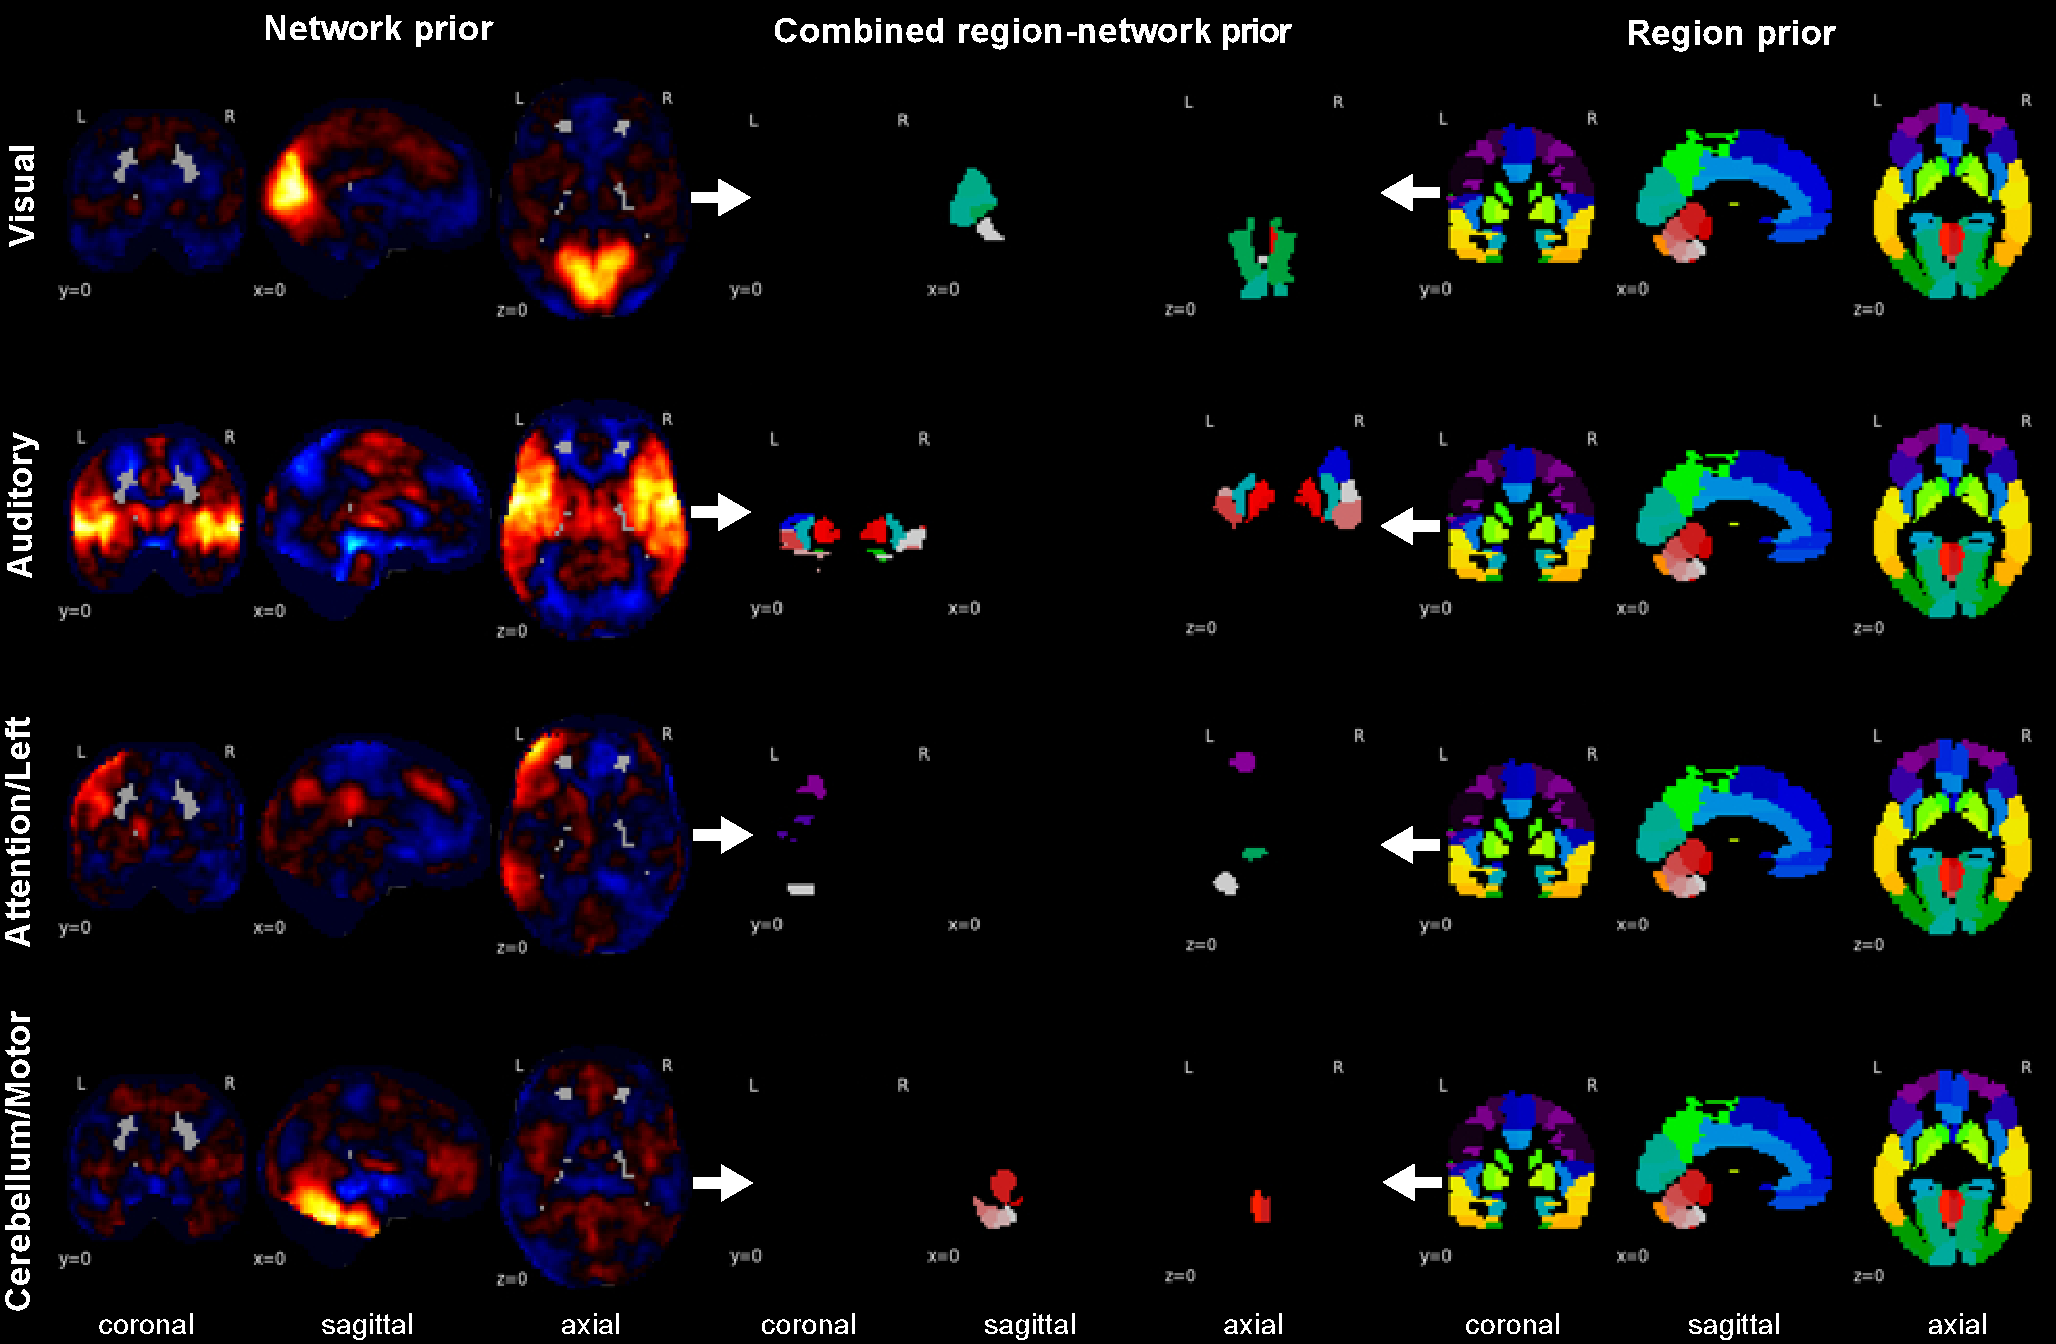
\includegraphics[width=1.00\textwidth]{figures/reg_net_prior.pdf}
\end{centering}
\vspace{-0.6cm}
\caption{\textbf{Building blocks of the region-network tree.}
Depicts neurobiological priors introduced into the supervised classification
by hierarchical structured sparsity.
\textit{Left:} Continuous, partially overlapping brain network priors
(\textit{hot-colored}, taken from \cite{smith2009})
accommodate the functional integration
perspective of brain organization.
\textit{Right:} Discrete, non-overlapping brain region priors
(\textit{single-colored}, taken from \cite{crad12})
accommodate the functional segregation perspective.
\textit{Middle:} These two types of predefined voxel groups are incorporated
into hierarchical priors of parent networks with their
descending region nodes.
\textit{Top to bottom:} Four examplary region-network priors
are shown, including
the early cortex that processes
visual and sound information from the environment,
a well-known attentional circuit in the left brain hemisphere,
and
the cerebellum that realizes motor behavior.
}
\label{fig_priors}
\end{figure}


\begin{figure}
\begin{centering}
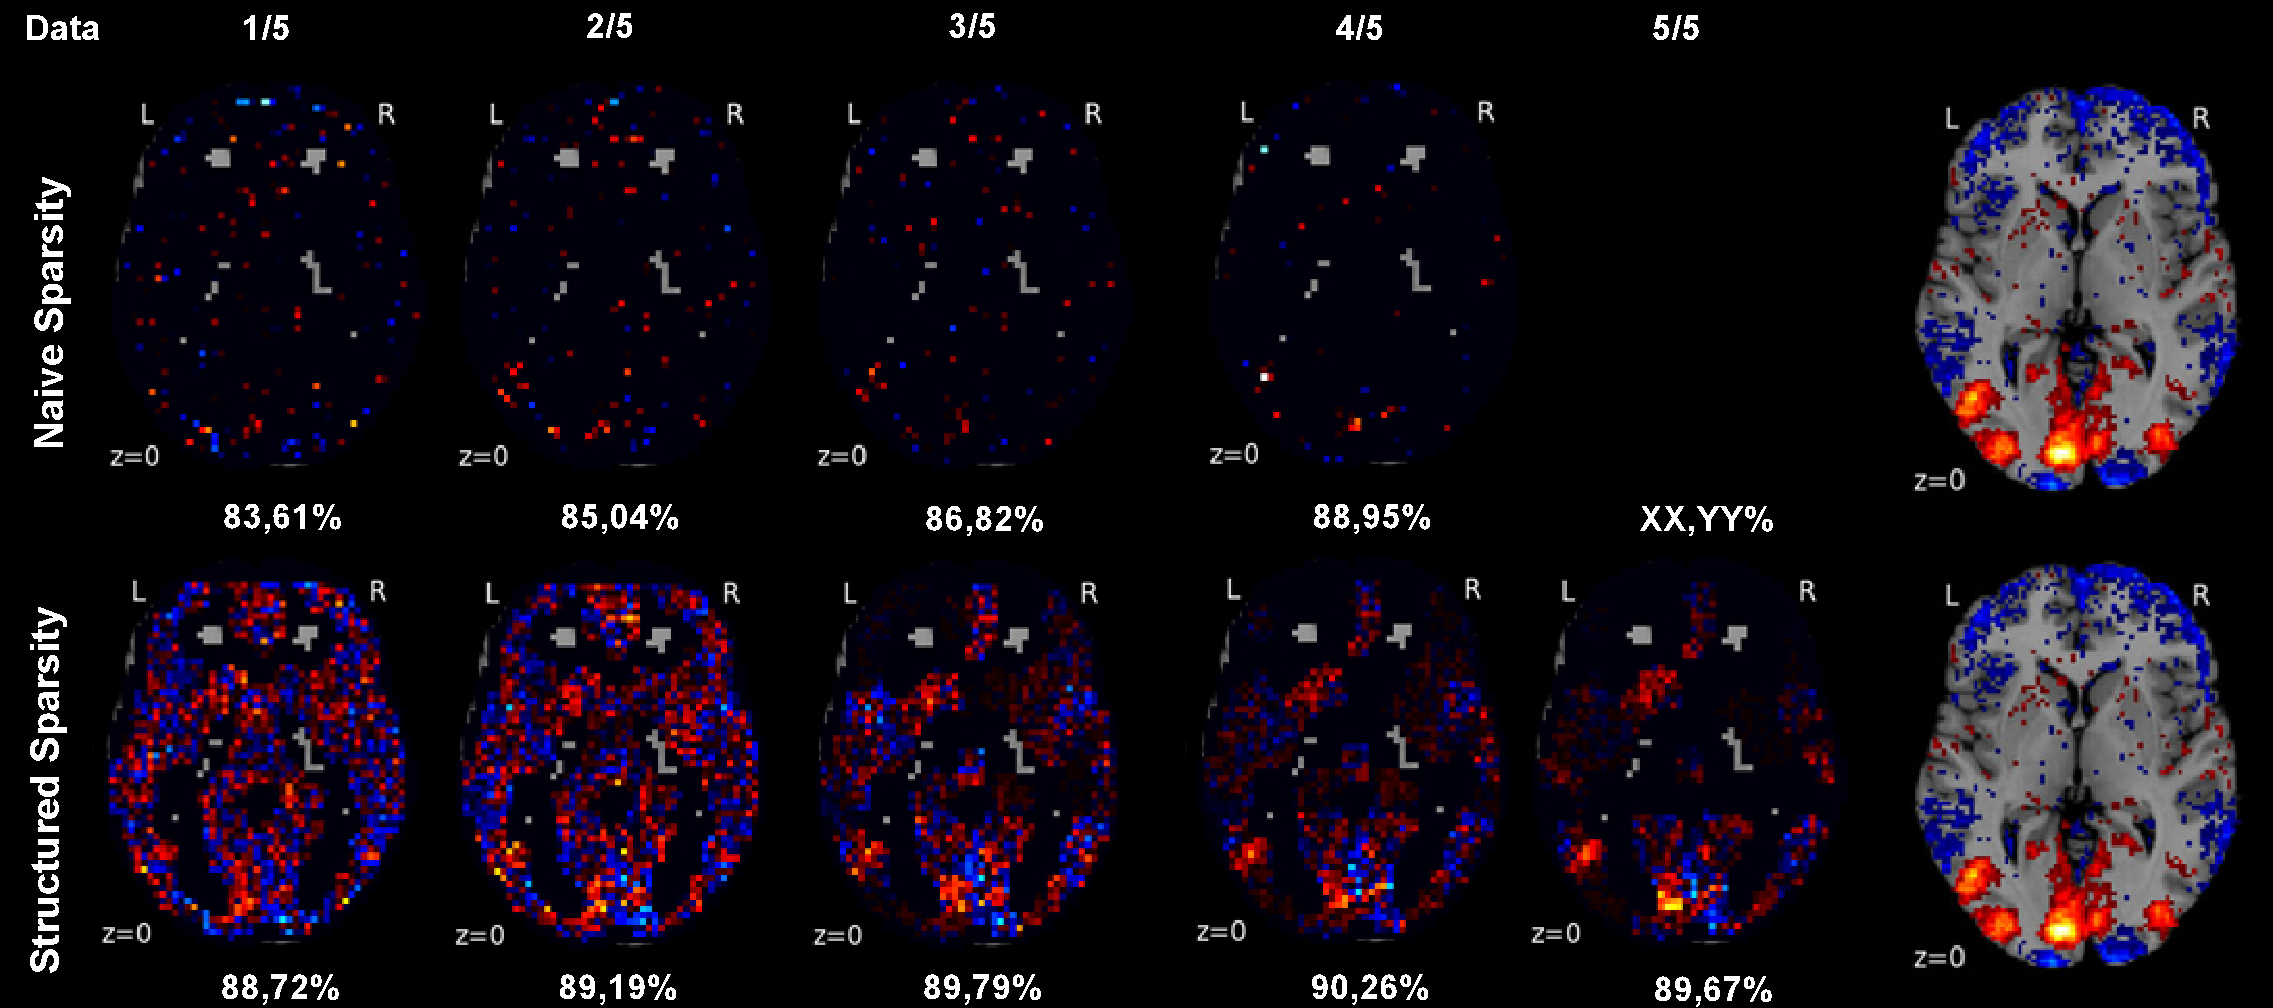
\includegraphics[width=1.00\textwidth]{figures/dataratio.pdf}
\end{centering}
\vspace{-0.6cm}
\caption{\textbf{Na\"ive versus informed sparse model selection
across training set sizes.}
Ordinary $\ell_1$-penalized logistic regression
(\textit{upper row})
is compared
to hierarchical-tree-penalized logistic regression
(\textit{lower row})
with increasing fraction
of the available training data (\textit{columns}).
For one example from 18 classes,
unthresholded coronal maps of model weights
are shown for comparison against
the class sample average
in the \textit{rightmost column}.
The corresponding 18-class (``View tools'')
out-of-sample accuracy
is given in percent.
%
In the data-scarce scenario,
typical for brain imaging,
hierarchical tree sparsity achieves
better support recovery with the biggest difference
in model performance.
%
In the data-rich scenario,
neurobiologically informed logistic regression
profits more from the increased information quantities than
neurobiologically naive logistic regression.
}
\label{fig_dataratio}
\end{figure}


\begin{figure}
\begin{centering}
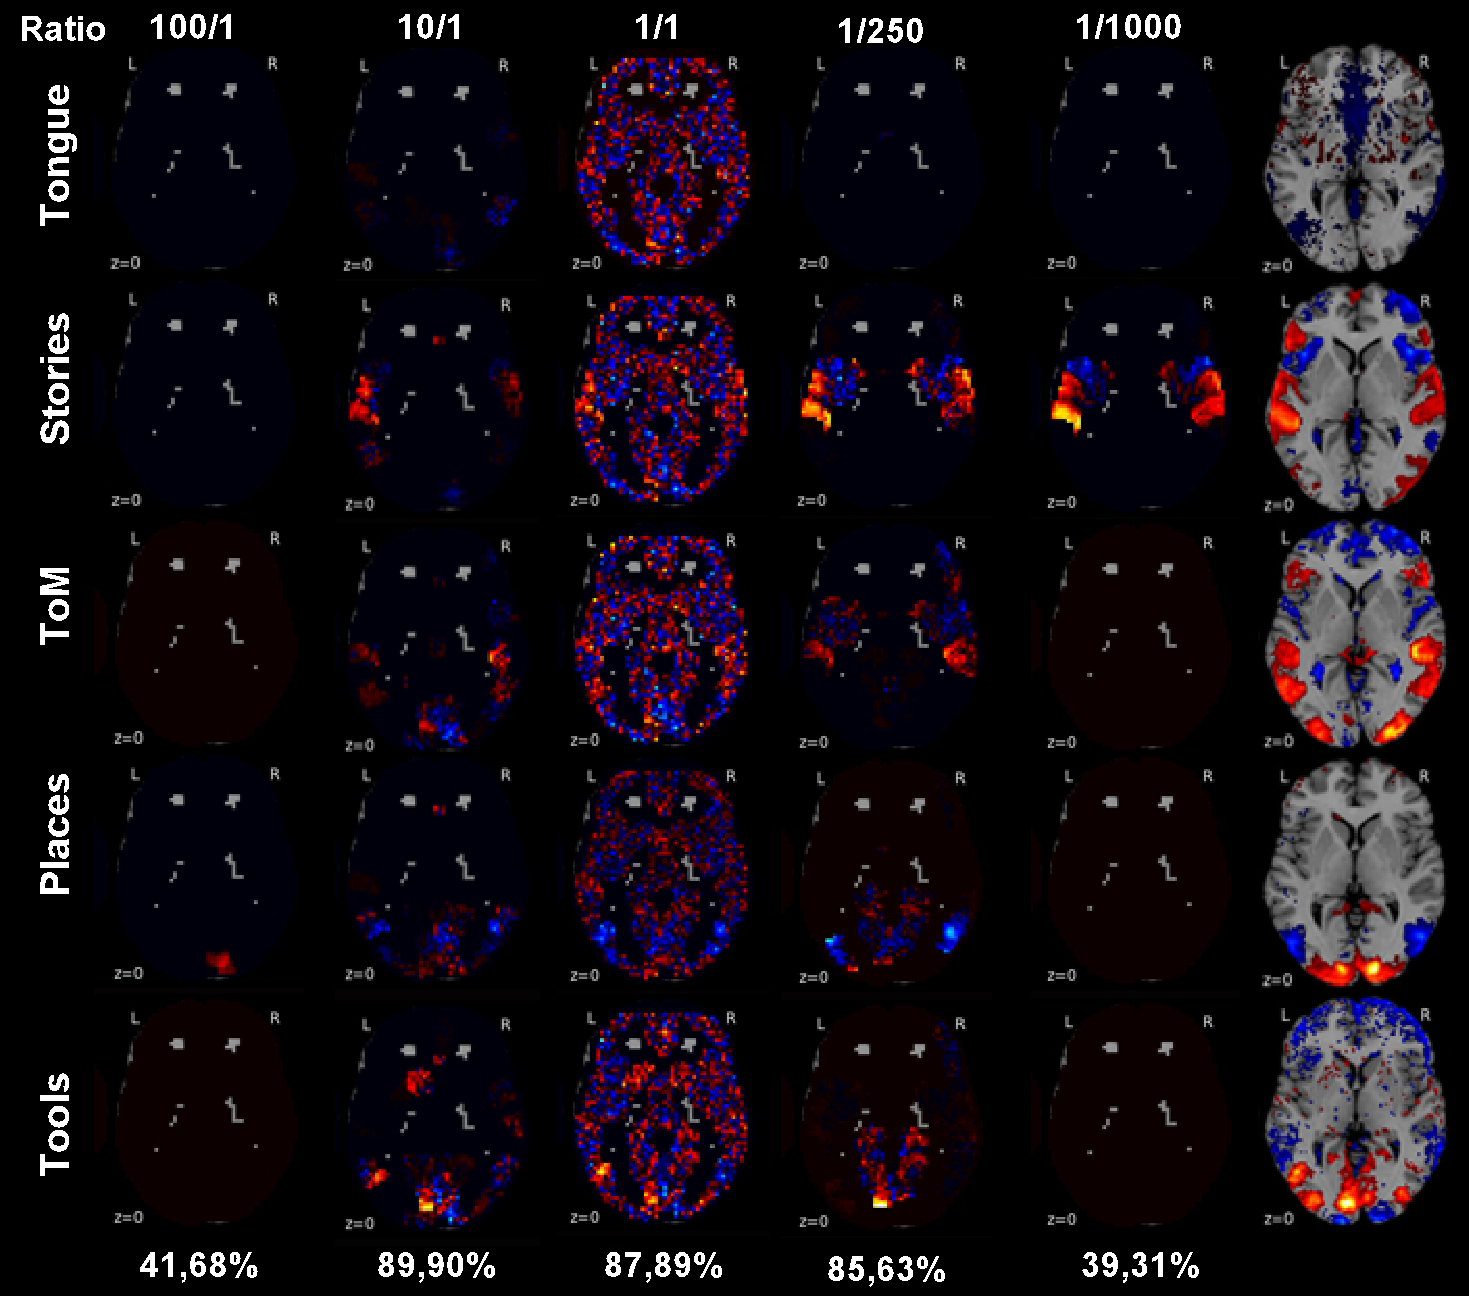
\includegraphics[width=1.00\textwidth]{figures/reg_net_ratio.pdf}
\end{centering}
\vspace{-0.6cm}
\caption{\textbf{Support recovery as a function of
region and network emphasis.}
The relative impact of the region and network priors
on model selection
is systematically varied against each other.
This region-network ratio (\textit{upper row}) weighted voxel groups
to priviledge sparse models in function space
that acknowledge known brain region neighborhoods
(\textit{left columns}) or
known brain networks compartments
(\textit{right columns}).
Among the 18 classes, the model weights are shown for the
tasks (\textit{from top to bottom}): tongue movement, listening stories,
taking somebody else's perspective (ToM, "theory of mind"),
as well as
viewing locations and tools.
The 18-class out-of-sample accuracy is indicated
on the \textit{bottom} and
the class-wise mean neural activty
in the \textit{rightmost column}.
%
Different emphasis on regions versus networks
in hierarchical structured sparsity can
yield essentially similar model performance.
%
Priviledging region versus network structure during model selection
recovers complementary aspects of the brain activity pattern.
%
Equal region and network emphasis yields more dispersed,
less interpretable predictive model choices.
}
\label{fig_ratio}
\end{figure}



\paragraph{Sample complexity of na\"ive versus informed sparse model selection.}
Subsequently, the sample complexity of
$\ell_1$-penalized and hierarchical-tree-penalized logistic regression
were quantitatively compared (Figure \ref{fig_dimred}).
Region-network priors should bias/guide model selection towards more
neurobiologically plausible classification estimators.
This should yield better out-of-sample generalization and
support recovery than
$\ell_1$-constrained logistic regression na\"ive to neurobiology
in the data-scarce and data-rich scenarios.
%
The HCP task data from 18 tasks was first divided into
90\% training set (i.e., 7584 maps) and
10\% test set (i.e., 842 maps).
Both learning algorithms were fed by the
training set that was subsampled to fractions of
25\% (X neural activity maps),
50\% (Y maps),
75\% (Z maps).
The estimators were submitted to a nested cross-validation scheme
for model selection and assessment.

In the inner CV layer, the logistic regression estimators
have been fitted in a one-versus-rest design that
distinguishes each class from
the respective other 17 classes
(number of maximal iterations=100, tolerance=$0.001$).

In the out CV layer, grid search



A grid of $\lambda$ candidates was searched between $10^-2$ and $10$
in 9 steps on a log scale.

evaluated on the allows same test set




\paragraph{Support recovery as a function of region and network emphasis.}








\section{Discussion}
Relevant structure in brain imaging data has long been
separately investigated
along two distinct organizational principles:
functional segregation into discrete brain regions
and functional integration by inter-regional brain networks.
%
This paper demonstrates the simultaneous exploitation of
both these neurobiological compartments
for sparse variable selection and high-dimensional prediction.
%
Introducing existing domain knowledge into model selection
naturally priviledges model hypotheses in the function space
that are most neurobiologically plausible.
%
The neurobiologically informed
hierarchical structured sparsity penalty is shown to enhance
model interpretability and generalization performance,
although these statistical goals are typically in conflict.




1) each voxel
We assume regions and networks but can estimate 
importance of each voxel.
neurobiologically motivated restrictions to
complexity circumvented the curse of dimensionality and allowed
for useful, simplified views on brain function.
previously laborious feature engineering / selection procedures


2) restrictions to complexity according to neurobiological facts
-> bias-variance tradeoff: negigible increase in bias but large decrease in variance
-> VC: decrease complexitiy capactiy -> better chance for generalization out of sample

guide model selection

3)
multiple comparisons problem has the curse of dimensionality
as its close correspondence in statistical learning
sparsity -> solves the curse at the estimation level

4) region-constrained or network-constrained model estimation
can lead to similar predictive performance



In the future,
the proposed regularization scheme can be used for various
learning tasks in systems neuroscience.
This includes supervised classification and regression
with one or several target variables.
%
Region-network sparsity priors could even be used to inform
unsupervised statistical estimators,
including principal component analysis
\cite{jenatton2009structured}
and
k-means clustering \cite{???}.
%
Additionally,
the structured sparsity penalty could be extended
from the spatial domain of neural activity to
spatiotemporally coherent neural activity patterns
\cite{gramfort2011tracking}.
%
Ultimately,
successful high-dimensional inference is
an important prerequisite
for prediction of diagnosis,
disease trajectories, and treatment responses
for personalized medicine in psychiatry and neurology
\cite{gabrieli2015prediction}.



\paragraph{Acknowledgment.}
{\small The research leading to these results has received funding from the
European Union Seventh Framework Programme (FP7/2007-2013)
under grant agreement no. 604102 (Human Brain Project).
Data were provided by the Human Connectome Project.
Further support was received from
the German National Academic Foundation (D.B.),
the German Research Foundation (BZ2/2-1 and BZ2/3-1 to D.B.),
and the MetaMRI associated team (B.T., G.V.).
}

  
\small
% \bibliographystyle{plainnat}
\bibliographystyle{splncs03}
\bibliography{paper_refs}



\end{document}
